\section{Natural Language Generation}

Natural Language Generation (NLG) is a sub-field of Natural Language Processing that attempts to generate sequences of words that resemble natural human languages. Traditionally, this was done either by using production rules of a pre-defined grammar, or by performing statistical analyses of existing human-written texts to predict sequences of words based on their occurrence probabilities. Markov-chain text generators are an example of the latter, popularized by their usage in parody text generation \cite{jelinek1985markov}.

This broad classification of problems has multiple applications include, and are not limited to:
\begin{itemize}
	\item Neural machine translation (NMT), in which the generation objective is to produce a semantically similar sentence in a target language, given a sentences in a source language.
	\item Dialogue generation, in which the objective is to produce a natural and syntactically correct response to the provided utterance.
	\item Text summarizaton, which eliminates superfluous and non-pertinent information in a body of text, to express the idea using fewer words.
	\item Data-to-text report generation, which utilizes structured data, sourced from a relational database format to fill out a text template.
\end{itemize}

\section{Recurrent Neural Networks}

Recurrent neural networks (RNNs) are a sub-class of artificial neural networks that can be considered a neural network equivalent to a Hidden Markov Model. Its units forms a directed graph that operates on a sequence of inputs when unrolled temporally. This makes them a useful tool for extracting features from arbitrary length sequences of input like audio or text. The features extracted at a given temporal point in an instance (sequence) is given by the below equation.
\begin{equation}
	P(w_1, \cdots, w_T) = \prod_{i=1}^T P(w_i | w_1, \cdots, w_{i−1})
\end{equation}

The language model is built in such a way that the features extracted from the sequence at epoch $t$ depend on the features observed during the epochs $0 \cdots t-1$. A graphical depiction of an unrolled RNN is shown in figure \ref{fig:recurrent-neural-network-unfold}.

\begin{figure}[ht]
	\centering
	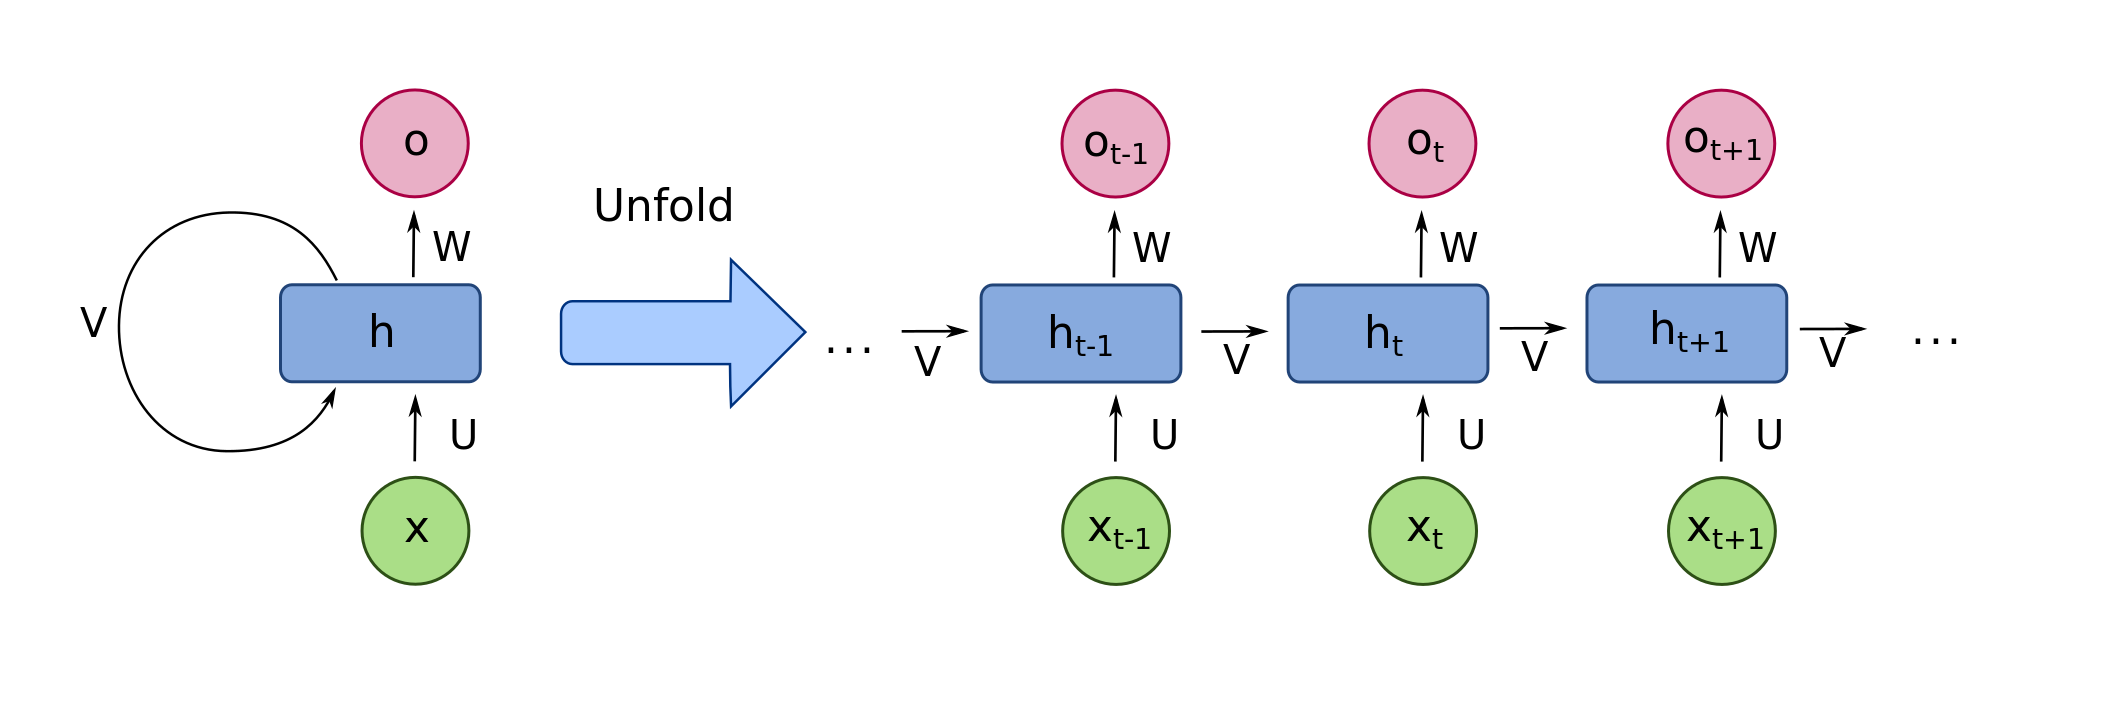
\includegraphics[width=\textwidth]{images/recurrent-neural-network-unfold}
	\imgsrc{\url{https://commons.wikimedia.org/wiki/File:Recurrent_neural_network_unfold.svg}}
	\caption{\label{fig:recurrent-neural-network-unfold} Unrolled RNN}
\end{figure}

The most recent and useful variants of recurrent units provide the ability to retain `memory' of the context in which the current features are to be considered. In the domain of language processing, this typically implies that the recurrent unit has a stored memory of the previously observed words in a sequence, and this property grants it the ability to learn context as part of the feature space.

The prominent variants of recurrent units used in neural networks to extract features from sequences using a memory mechanism, are Long Short-Term Memory (LSTM) units \citep{gers2001lstm} and Gated Recurrent units (GRU) \citep{chung2014empirical}.

Recurrent networks in the domain of natural language processing is used frequently for both natural language understanding (NLU) tasks, as well natural language generation (NLG) tasks. Similar to the manner in which recurrent networks can extract features from arbitrarily long sequences of vectorized text, they can also be used to produce text sequences from a unit vector representation of text, as represented in Figure \ref{fig:rnn-nmt}.

This is achieved by conditioning the generation of the first word of text either on some latent variable produced by a model, or by sampling from a generative distribution, and conditioning the generation of each subsequently predicted word on the word that was predicted in the previous time-step, until the model predicts an end-of-sentence (EOS) token.

\begin{figure}[ht]
	\centering
	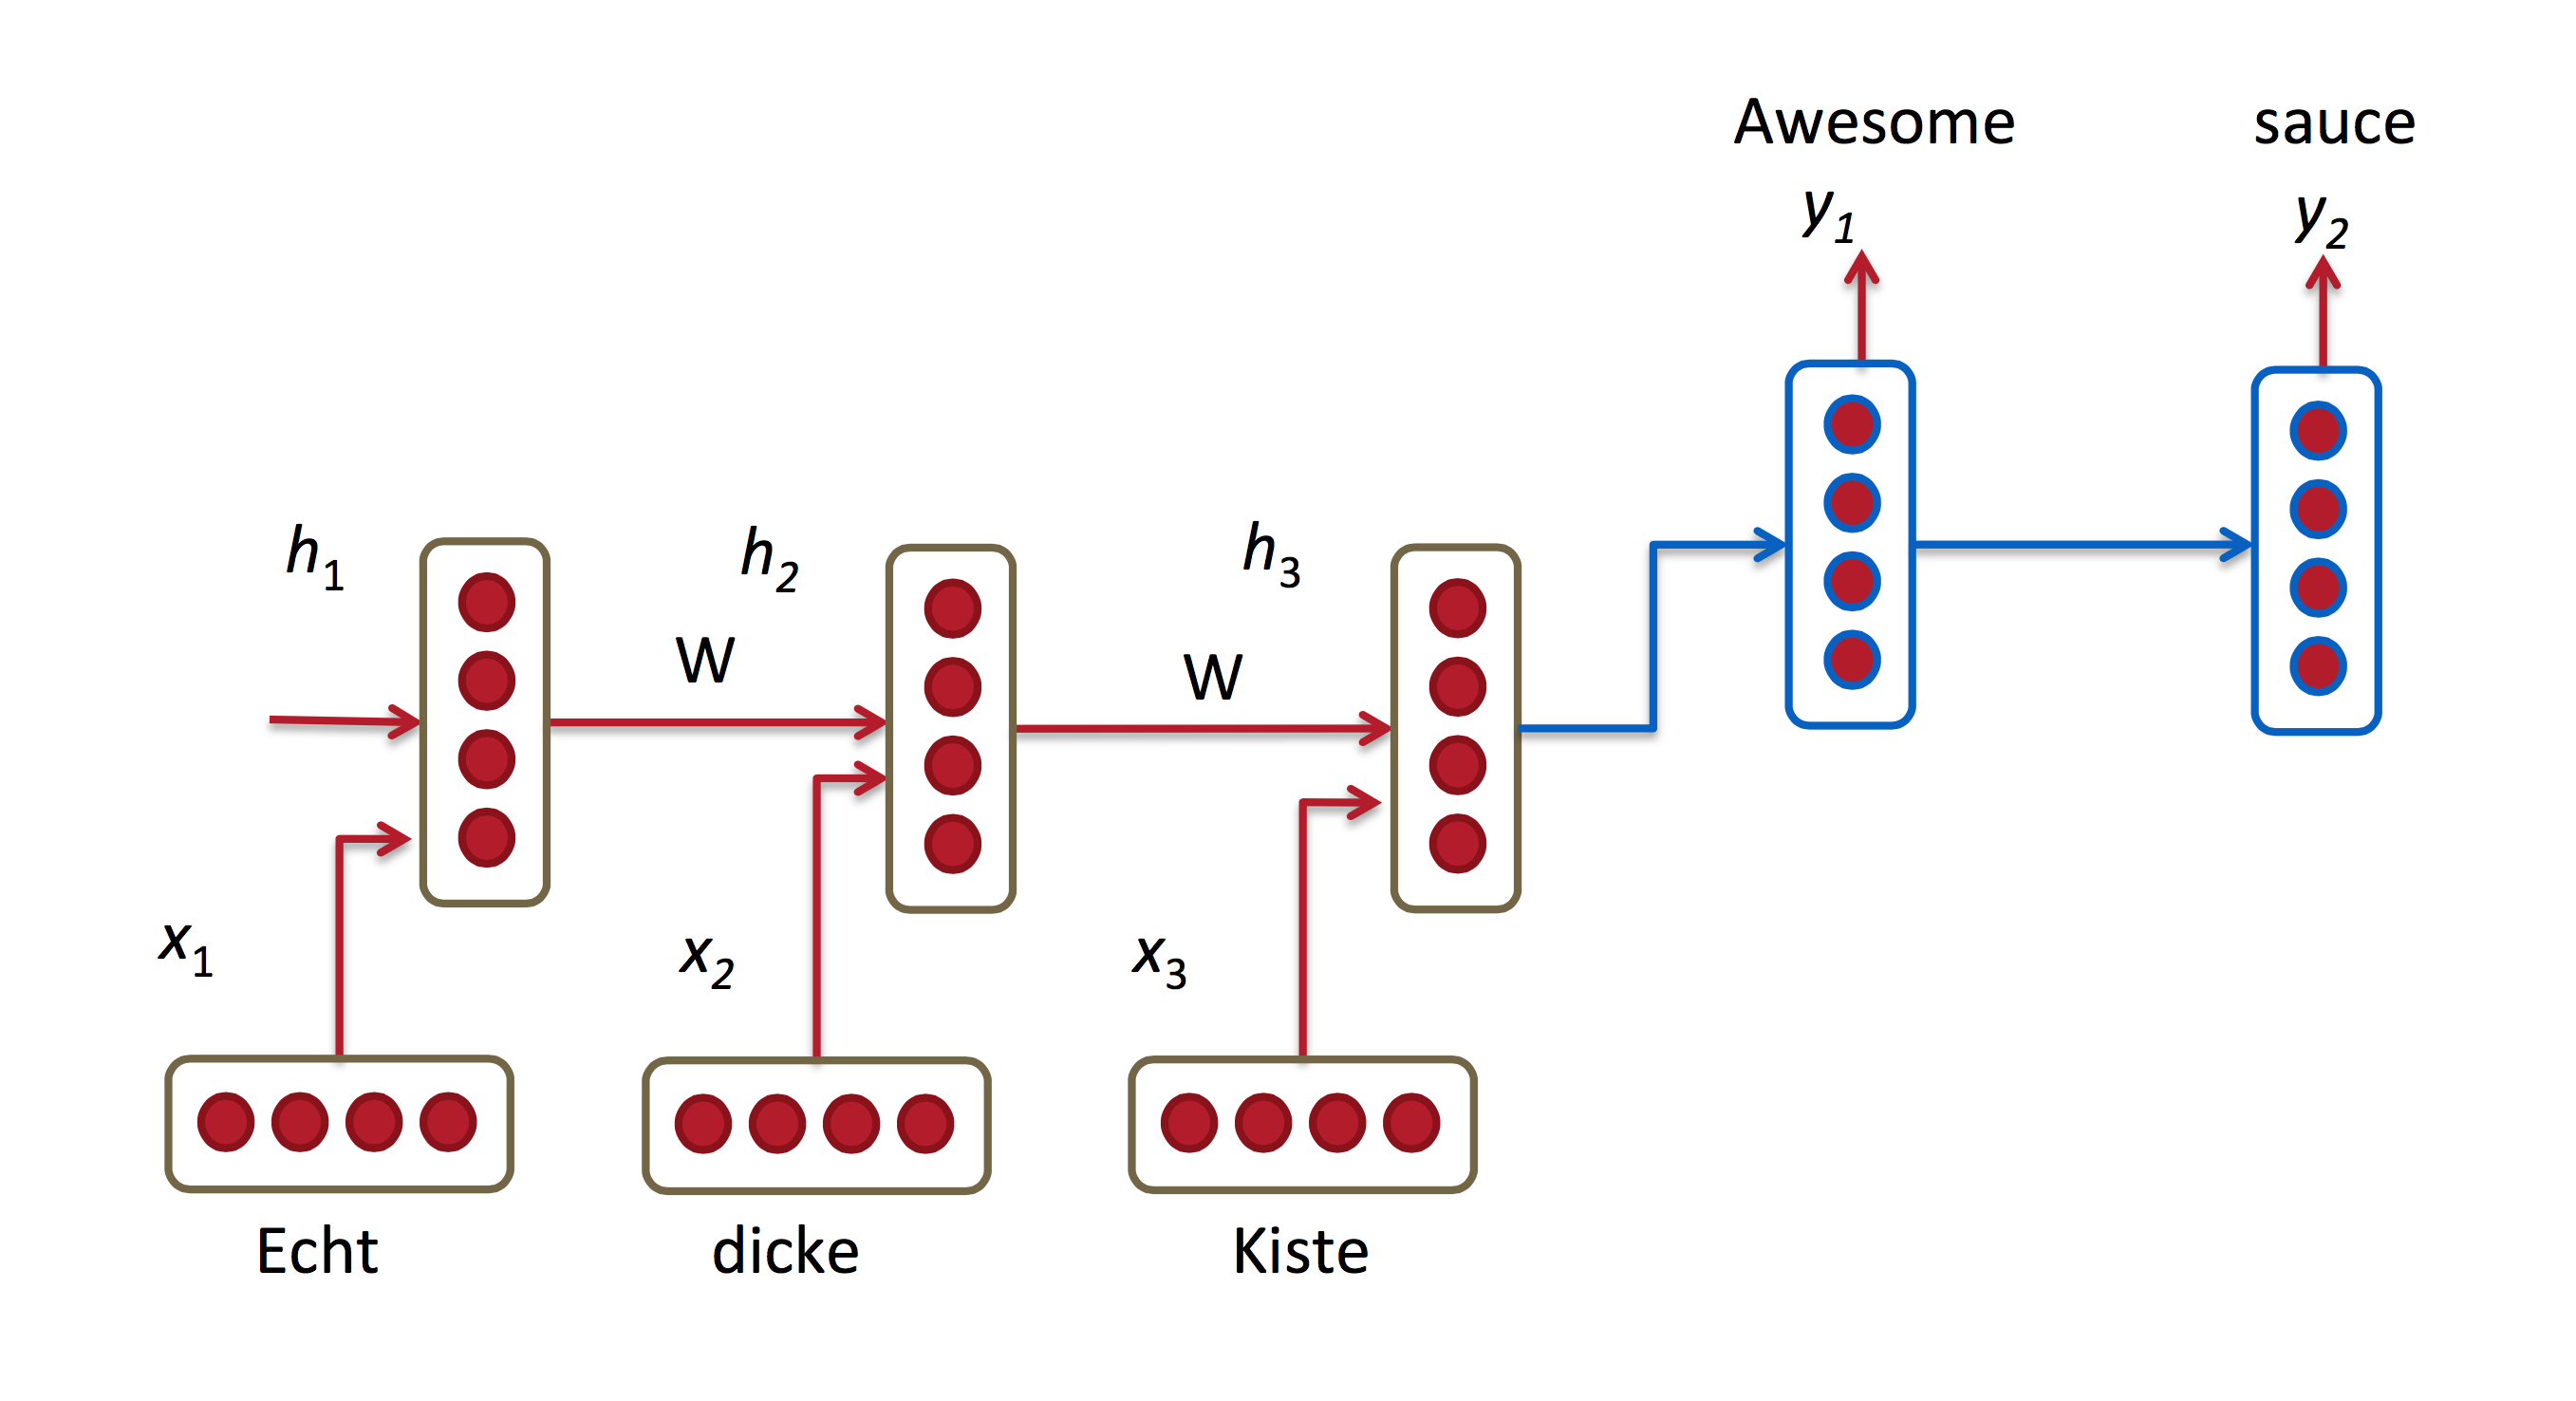
\includegraphics[width=\textwidth]{images/rnn-nmt}
	\imgsrc{\url{http://www.wildml.com/2015/09/recurrent-neural-networks-tutorial-part-1-introduction-to-rnns}}
	\caption{\label{fig:rnn-nmt} Recurrent Network Encoder-Decoder}
\end{figure}

\section{Autoencoders}

Autoencoders are models that are parameterized to convert arbitrary data into a latent representation (encoder), and recover the original data back from the latent representation (decoder). In this setup, the degrees of freedom for the latent representation is usually much smaller than that of the actual data. A simple autoencoder architecture is depicted in Figure \ref{fig:autoencoder-structure}.

\begin{figure}[ht]
	\centering
	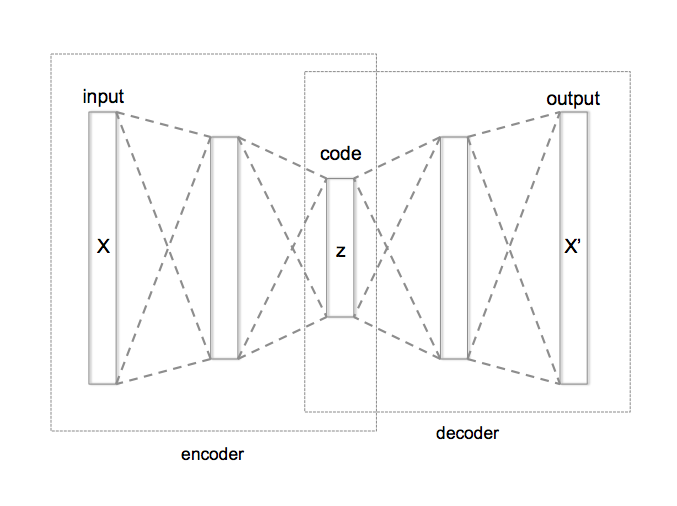
\includegraphics[width=\textwidth]{images/autoencoder-structure}
	\imgsrc{\url{http://mlexplained.com/2017/12/28/an-intuitive-explanation-of-variational-autoencoders-vaes-part-1}}
	\caption{\label{fig:autoencoder-structure} Autoencoder Architecture}
\end{figure}

By training a model to do this, two objectives can be achieved simultaneously:
\begin{itemize}
	\item The encoder weights of the model could be used extract the most salient features of the data in a compressed representation, which is a friendlier format for downstream processing or learning algorithms. \citep{hinton2006reducing}
	\item The decoder weights of the model could be used as a generator. Given that we can sample from the distribution of the existing latent representations learnt, or from a pre-defined prior (in a variational autoencoder), we can generate plausible novel data.
\end{itemize}

In the context of natural language the encoder can be utilized as a sentence-encoding feature-extractor and the decoder can be utilized as a generative model. Autoencoders are also used for being able to de-noise data given pairs of noisy and regular data, by learning a de-noising function. These properties make autoencoders a good framework to utilize to implement sequence-to-sequence models, where both the encoder and decoder weights of the network are parameterized by recurrent neural networks.

\subsection{Variational Autoencoders}

Variational encoders (VAEs) \citep{kingma2013auto} are a probabilistic variant of autoencoders. The general structure of a VAE is the same as that of a deterministic autoencoder, with an encoder that learns a compressed latent space and a decoder that learns a function to map the latent space into the original data. A simple VAE architecture is depicted in Figure \ref{fig:vae-structure}.

\begin{figure}[ht]
	\centering
	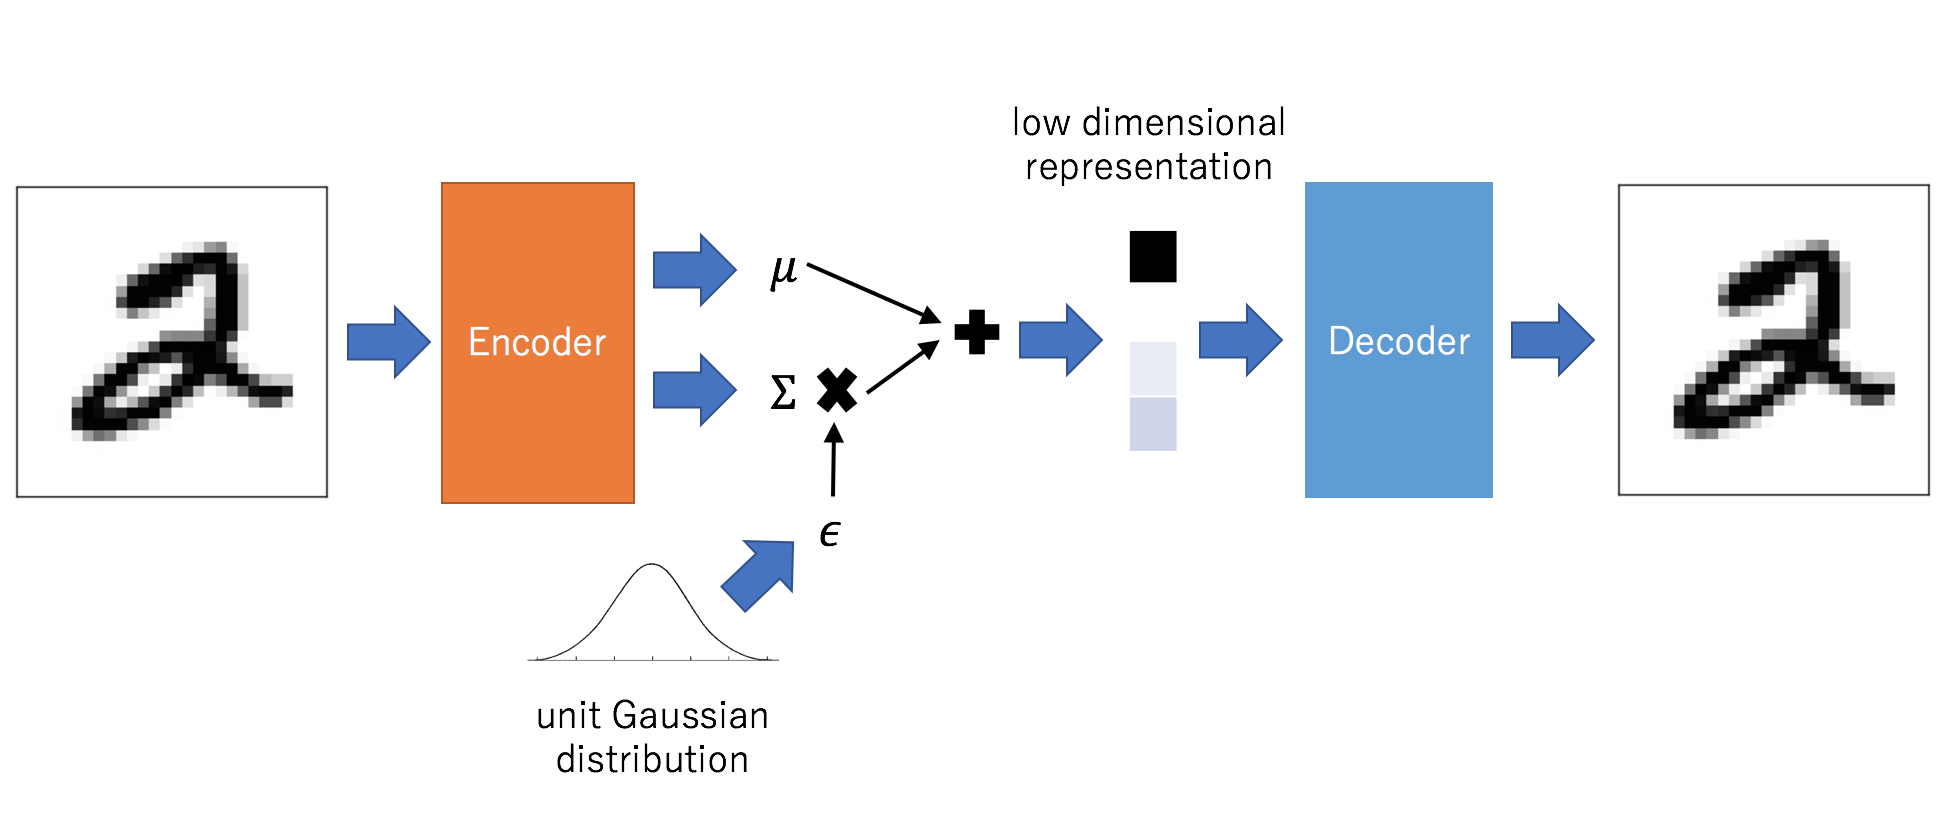
\includegraphics[width=\textwidth]{images/vae-structure}
	\imgsrc{\url{http://mlexplained.com/2017/12/28/an-intuitive-explanation-of-variational-autoencoders-vaes-part-1}}
	\caption{\label{fig:vae-structure} VAE Architecture}
\end{figure}

In contrast to the deterministic autoencoder we observe that a variational inference networks autoencoder learns representations of both the mean and variance latent spaces. The method requires placing conjugate priors on the mean and variance of the unknown latent representation. The encoder then tries to learn the approximate posterior distribution. This family of distributions used for this purpose are Gaussian.

In addition to the reconstruction loss that a deterministic autoencoder uses, a metric of distance is used to evaluate how closely between the learned representations of mean and variance resemble a Gaussian distribution with mean 0 and unit variance. The Kullback-Leibler (KL) divergence \citep{kullback1951information} is used to penalize learned representations that do not resemble the prior. However, we cannot compute the KL directly. Instead we compute an alternative objective that is equivalent to the KL upto an added constant. This is called the evidence lower-bound (ELBO). The ELBO objective maximized in a variational autoencoder model is given below:

\begin{equation}
	ELBO(q) = \mathbb{E}_{q(z)} [(\log(p(x|z))] - \mathbb{KL}(q(z)||p(z))
\end{equation}

Simultaneously, for the decoding step, we sample from the prior, utilizing the re-parameterization trick to ensure that the model remains differentiable. As a result the decoder is trained as a generative network that can randomly sample from the prior and generate plausible data similar to the input distribution. The decoder being able to act as a generative model independently is what sets a VAE apart from a generative model.

\section{Sequence to Sequence Modeling}

Also abbreviated in the literature as Seq2Seq, this is a class of models that learns functions that map from one sequence to another. First introduced by \cite{sutskever2014sequence}, the general premise of sequence to sequence has been a flexible framework for modelling transformations made to arbitrary length sequences. In the natural language processing community, the main tasks that benefit from the encoder-decoder framework are neural machine translation, dialogue modeling, question answering for which there exists two distinct distributions of data, and the model is trained to learn the mapping from one to the other.

The paper defines a sequence-to-sequence model as on that learns the below function to map a sequence of inputs $x_1, ... , x_T$ to a sequence of outputs $y_1, ... , y_{T′}$, where the initial state $h$ is set to the hidden LSTM representation of $x_1, ... , x_T$.

\begin{equation}
	p(y_1, ... , y_{T′} | x_1, ... , x_T) =	\prod_{t=1}^T p(y_t | h, y_1, ... , y_{t−1})
\end{equation}

This makes the Seq2Seq model an ideal framework using which one can implement solutions to several natural language generation tasks like neural machine translation, dialogue generation, text summarizaton etc.

\section{Adversarial Networks}

\cite{goodfellow2014generative} present a new model that utilizes the idea of a game-theoretic competition between the generative model which is a decoder, and a discriminative model which is usually a classifier or regressor. The general idea is to train the adversary to be able to discriminate between the distributions that the generator model is trying to produce and a true distribution, that it the generator trying to mimic.

\begin{figure}[ht]
	\centering
	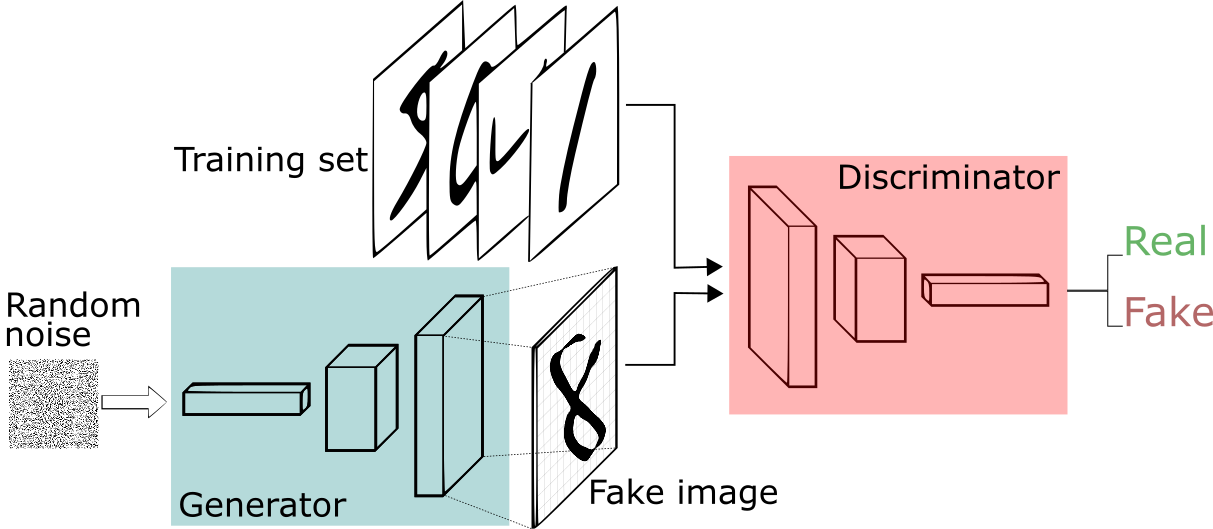
\includegraphics[width=\textwidth]{images/gans}
	\imgsrc{\url{https://deeplearning4j.org/generative-adversarial-network}}
	\caption{\label{fig:gans} GAN Architecture}
\end{figure}

In the original formulation of adversarial training, which involves using a binary classifier, the generator learns weights to map a randomly initialized latent variable $z$ to a data distribution $x$ that it is unaware of. The discriminator is trained using the true distribution and samples generated by the generative model, and it's objective is to discriminate the true samples from the generated samples. The generator on the other hand, attempts to maximize the discriminator's classification error, thereby producing plausible samples that mimic the true distribution.

This property of the generator model parameters possess, of translating random noise into plausible data samples are used in areas of research within computer vision and natural language processing to produce novel data. Also adversarial learning as a principle is a great tool to ensure that known partial information present in the latent space is disentangled from any arbitrarily chosen sub-space.

We utilize adversarial learning in our model to assist with the disentanglement of style labels.


\section{Image Style Transfer}

The idea of neural style transfer in the was originally proposed by \cite{gatys2016image}. In the task described in the paper, the authors use two distinct images as input. The first image contributes the content, and the second contributes the style. The objective is to generate a final image that contains all of the physical objects visible in the first image, but depicted by the style (hue, brush strokes, texture etc.) visible in the second.

\begin{figure}[ht]
	\centering
	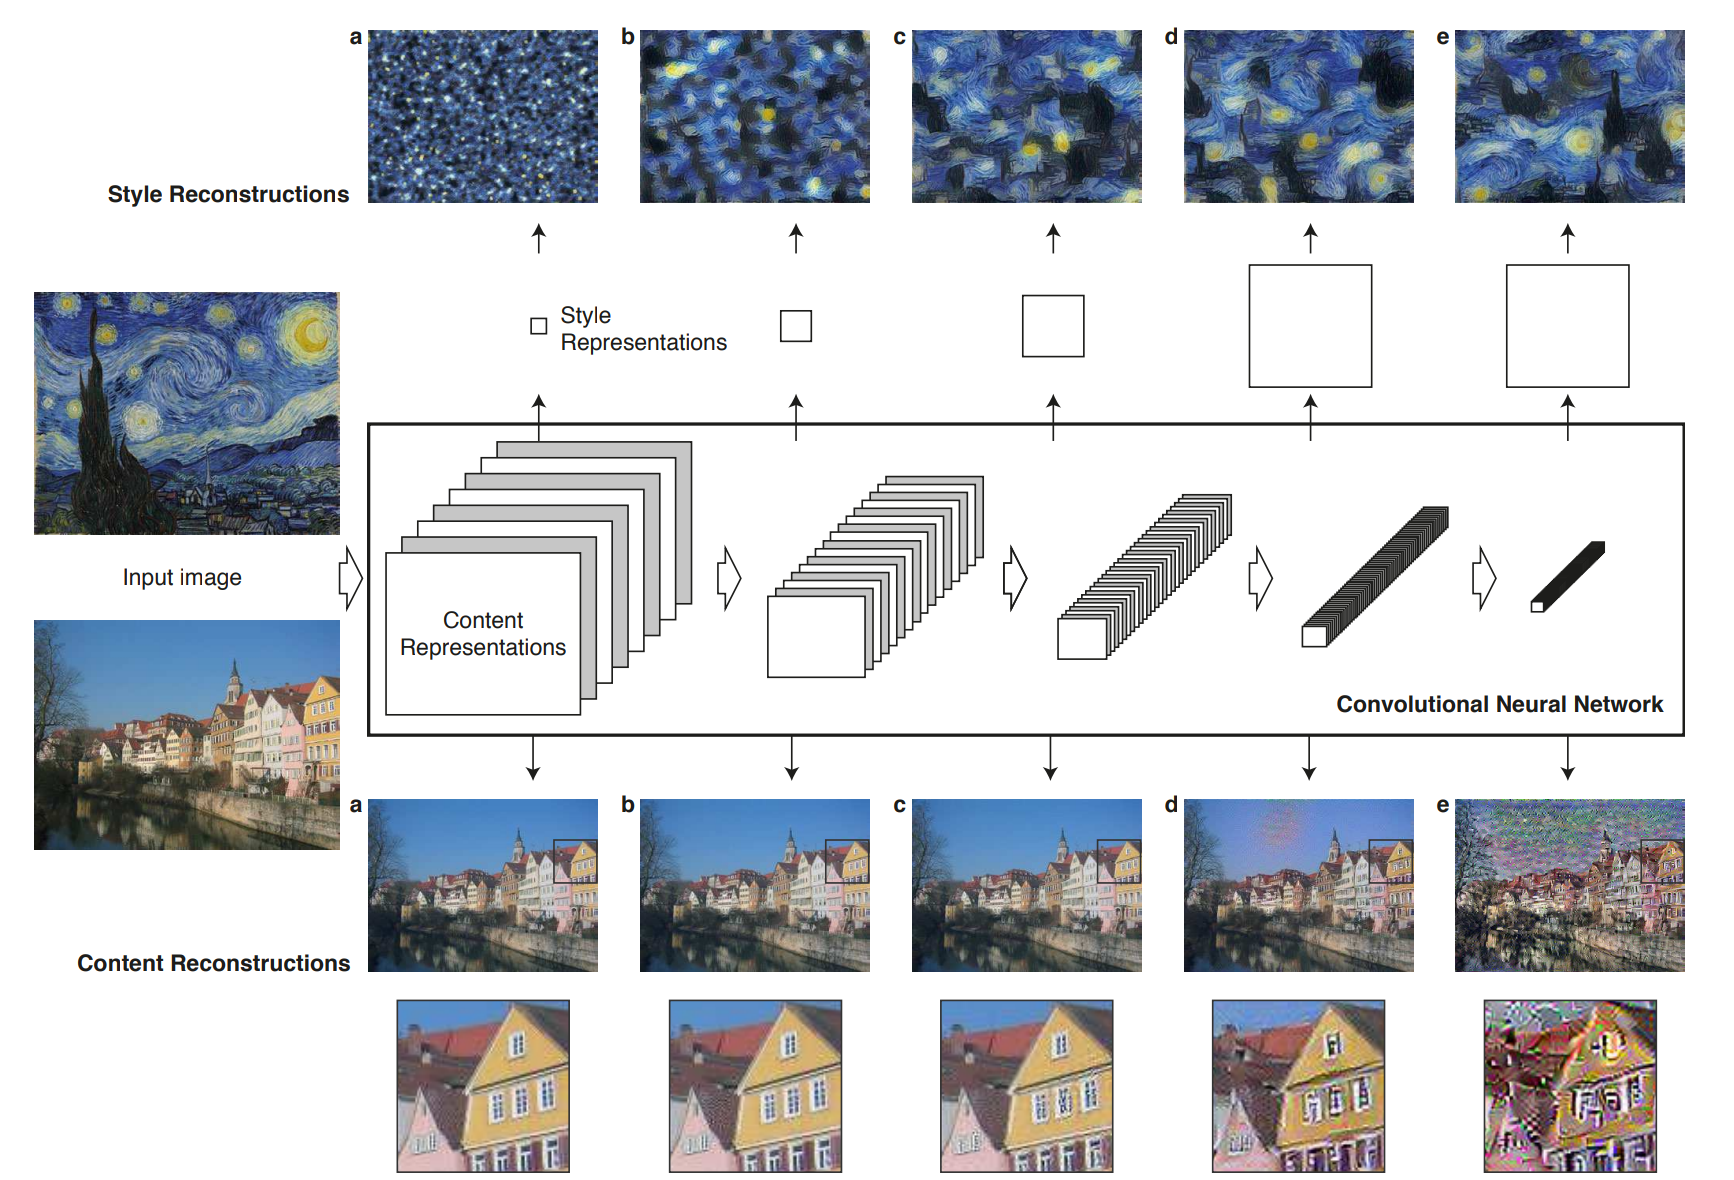
\includegraphics[width=\textwidth]{images/image-style-transfer.png}
	\imgsrc{\cite{gatys2016image}}
	\caption{\label{fig:image-style-transfer} Artistic Style Transfer in Images}
\end{figure}

The features, as with most of the state-of-the-art image processing techniques, are extracted from the images using Convolutional Neural Networks (CNNs) \citep{lecun1998gradient}, the deep neural network variants of which have been widely successful at image recognition tasks such as object recognition in the ImageNet data-set \cite{krizhevsky2012imagenet}.

As depicted in Figure \ref{fig:image-style-transfer}, subsequent layers of the CNN learn incrementally higher level features in both the style image and the content image. These learned features for the style and content images are stored for uture use. To generate the final image, the authors begin with a random white noise image. This image is passed through both networks, the parameters of which extract both it's style features and it's content features.

This model uses two training objectives:
\begin{itemize}
	\item Minimize the the element-wise mean squared difference between the style features computed for the style image and the white-noise image
	\item Minimize the the mean squared difference between the content features of the content image and the white noise image, as shown in the below equations.
\end{itemize}

The overall training loss is a linear combination of the above objectives, and is used to iteratively modify the white-noise image until it the style features of the style image and the content features of the content image.

The next chapter builds on the fundamentals established in this one, and discusses previous attempts at neural disentanglement in the context of linguistic style transfer as well as methods that do not use disentanglement as the basis of the style transfer model.
